\documentclass[tikz,border=12pt]{standalone}
\usepackage[T1]{fontenc}
\usepackage{mathpazo}
\usepackage{amsmath,amssymb}
\usetikzlibrary{arrows.meta, positioning, calc, fit, decorations.pathreplacing}

\definecolor{stblue}{HTML}{7B97AD}
\definecolor{rwgold}{HTML}{B8995E}
\definecolor{sage}{HTML}{7A9A7E}
\definecolor{dkbrown}{HTML}{3D3530}
\definecolor{wmgray}{HTML}{7B7067}
\definecolor{cream}{HTML}{F9F6F0}
\definecolor{border}{HTML}{D4C9B8}
\definecolor{terracotta}{HTML}{C47A6A}
\definecolor{lavender}{HTML}{907EA0}

\begin{document}
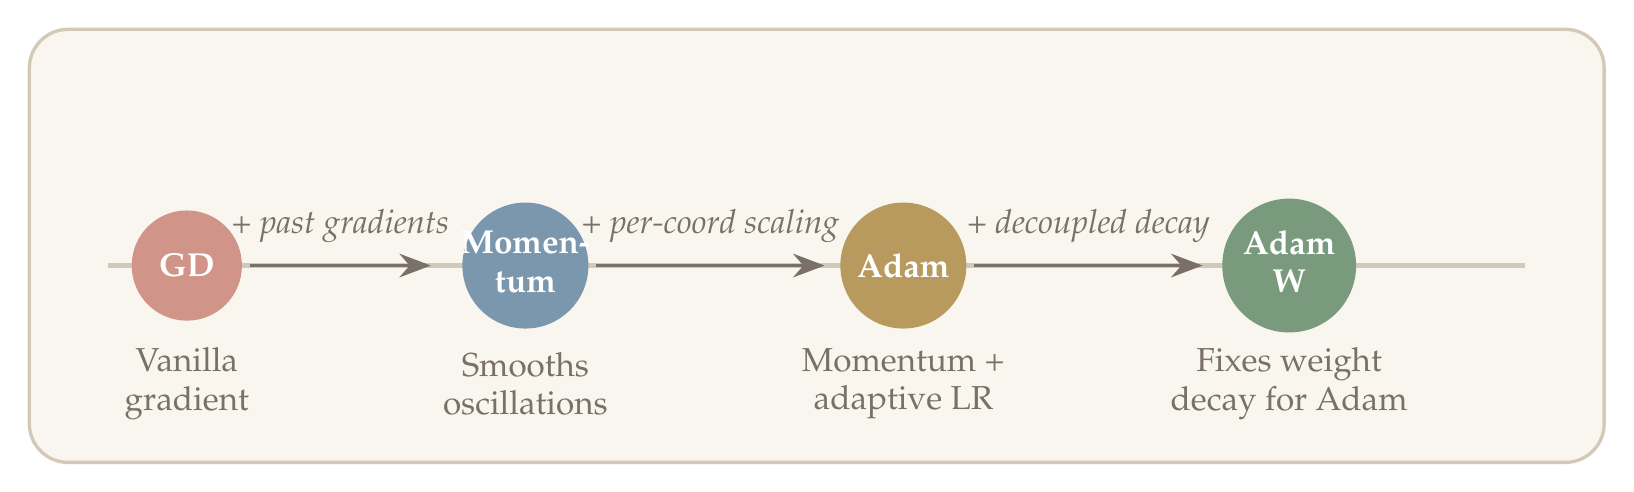
\begin{tikzpicture}[>={Stealth[length=4mm, width=3mm]}, line width=1.5pt]

% Background
\fill[cream, rounded corners=14pt] (-0.5,-2.5) rectangle (19.5,3.0);
\draw[border, line width=1.2pt, rounded corners=14pt] (-0.5,-2.5) rectangle (19.5,3.0);

% Timeline line
\draw[border, line width=1.5pt] (0.5,0) -- (18.5,0);

% GD node
\fill[terracotta!80] (1.5,0) circle (0.7);
\node[text=white, font=\large\bfseries] at (1.5,0) {GD};
\node[text=wmgray, font=\large, align=center] at (1.5,-1.5) {Vanilla\\gradient};

% Arrow GD -> Momentum
\draw[wmgray, ->, line width=1.2pt] (2.3,0) -- (4.6,0);
\node[text=wmgray, font=\large\itshape, above] at (3.45,0.15) {+ past gradients};

% Momentum node
\fill[stblue] (5.8,0) circle (0.8);
\node[text=white, font=\large\bfseries, align=center] at (5.8,0.05) {Momen-\\tum};
\node[text=wmgray, font=\large, align=center] at (5.8,-1.5) {Smooths\\oscillations};

% Arrow Momentum -> Adam
\draw[wmgray, ->, line width=1.2pt] (6.7,0) -- (9.6,0);
\node[text=wmgray, font=\large\itshape, above] at (8.15,0.15) {+ per-coord scaling};

% Adam node
\fill[rwgold] (10.6,0) circle (0.8);
\node[text=white, font=\large\bfseries] at (10.6,0) {Adam};
\node[text=wmgray, font=\large, align=center] at (10.6,-1.5) {Momentum +\\adaptive LR};

% Arrow Adam -> AdamW
\draw[wmgray, ->, line width=1.2pt] (11.5,0) -- (14.4,0);
\node[text=wmgray, font=\large\itshape, above] at (12.95,0.15) {+ decoupled decay};

% AdamW node
\fill[sage] (15.5,0) circle (0.85);
\node[text=white, font=\large\bfseries, align=center] at (15.5,0.05) {Adam\\W};
\node[text=wmgray, font=\large, align=center] at (15.5,-1.5) {Fixes weight\\decay for Adam};

\end{tikzpicture}
\end{document}
